%-------------------------------------------------------------------------------
%  AUTEUR : Boukary OUEDRAOGO
%  SUJET  : Synthèse de cours Entreposage et fouille de données
%  DATE DE CREATION : 23/12/2021
%-------------------------------------------------------------------------------
\documentclass{article}\usepackage[]{graphicx}\usepackage[]{color}
% maxwidth is the original width if it is less than linewidth
% otherwise use linewidth (to make sure the graphics do not exceed the margin)
\makeatletter
\def\maxwidth{ %
  \ifdim\Gin@nat@width>\linewidth
    \linewidth
  \else
    \Gin@nat@width
  \fi
}
\makeatother

\definecolor{fgcolor}{rgb}{0, 0, 0}
\makeatletter
\@ifundefined{AddToHook}{}{\AddToHook{package/xcolor/after}{\definecolor{fgcolor}{rgb}{0, 0, 0}}}
\makeatother
\newcommand{\hlnum}[1]{\textcolor[rgb]{0.69,0.494,0}{#1}}%
\newcommand{\hlstr}[1]{\textcolor[rgb]{0.749,0.012,0.012}{#1}}%
\newcommand{\hlcom}[1]{\textcolor[rgb]{0.514,0.506,0.514}{\textit{#1}}}%
\newcommand{\hlopt}[1]{\textcolor[rgb]{0,0,0}{#1}}%
\newcommand{\hlstd}[1]{\textcolor[rgb]{0,0,0}{#1}}%
\newcommand{\hlkwa}[1]{\textcolor[rgb]{0,0,0}{\textbf{#1}}}%
\newcommand{\hlkwb}[1]{\textcolor[rgb]{0,0.341,0.682}{#1}}%
\newcommand{\hlkwc}[1]{\textcolor[rgb]{0,0,0}{\textbf{#1}}}%
\newcommand{\hlkwd}[1]{\textcolor[rgb]{0.004,0.004,0.506}{#1}}%
\let\hlipl\hlkwb

\usepackage{framed}
\makeatletter
\newenvironment{kframe}{%
 \def\at@end@of@kframe{}%
 \ifinner\ifhmode%
  \def\at@end@of@kframe{\end{minipage}}%
  \begin{minipage}{\columnwidth}%
 \fi\fi%
 \def\FrameCommand##1{\hskip\@totalleftmargin \hskip-\fboxsep
 \colorbox{shadecolor}{##1}\hskip-\fboxsep
     % There is no \\@totalrightmargin, so:
     \hskip-\linewidth \hskip-\@totalleftmargin \hskip\columnwidth}%
 \MakeFramed {\advance\hsize-\width
   \@totalleftmargin\z@ \linewidth\hsize
   \@setminipage}}%
 {\par\unskip\endMakeFramed%
 \at@end@of@kframe}
\makeatother

\definecolor{shadecolor}{rgb}{.97, .97, .97}
\definecolor{messagecolor}{rgb}{0, 0, 0}
\definecolor{warningcolor}{rgb}{1, 0, 1}
\definecolor{errorcolor}{rgb}{1, 0, 0}
\makeatletter
\@ifundefined{AddToHook}{}{\AddToHook{package/xcolor/after}{
\definecolor{shadecolor}{rgb}{.97, .97, .97}
\definecolor{messagecolor}{rgb}{0, 0, 0}
\definecolor{warningcolor}{rgb}{1, 0, 1}
\definecolor{errorcolor}{rgb}{1, 0, 0}
}}
\makeatother
\newenvironment{knitrout}{}{} % an empty environment to be redefined in TeX

\usepackage{alltt}
%-------------------------------------------------------------------------------
%                  IMPORT OF ALL NEEDED PACKAGES
%-------------------------------------------------------------------------------
\usepackage[utf8]{inputenc}
\usepackage[french]{babel}
\usepackage[left=2.5cm,right=2.5cm,top=2cm,bottom=2cm]{geometry}
\usepackage[colorlinks=true,linkcolor=black,anchorcolor=black,citecolor=black,filecolor=black,menucolor=black,runcolor=black,urlcolor=black]{hyperref} 
\usepackage[T1]{fontenc} % Font encoding
\usepackage{graphicx}
\graphicspath{{Images/}}
\usepackage{eso-pic} 
\usepackage{subfig} 
\usepackage{caption} 
\usepackage{transparent}
\usepackage{amsmath}
\usepackage{amsthm}
\usepackage{bm}
\usepackage[overload]{empheq}  
\usepackage{tabularx}
\usepackage{longtable}
\usepackage{colortbl}
\usepackage{cleveref}
\usepackage[square, numbers, sort&compress]{natbib} 
\bibliographystyle{plain} 
\usepackage{appendix}
\usepackage{enumitem}
\usepackage{amsthm,thmtools}
%\usepackage[table]{xcolor}
\usepackage{comment} % Comment part of code
\usepackage{fancyhdr} % Fancy headers and footers
\usepackage{lmodern}
\usepackage{tcolorbox} 
\usepackage{amsmath,amsfonts,amssymb}
\usepackage{pgfplots,tikz}
\usetikzlibrary{matrix,chains,positioning,decorations.pathreplacing,arrows,fit}
\usepackage{enumitem}  
\usepackage[normalem]{ulem}
%fonts change 
\usepackage[charter]{mathdesign}
\tcbuselibrary{skins,breakable,xparse}
\usepackage{shadowtext}
\usepackage[explicit]{titlesec}
\usepackage{setspace}
\setstretch{1.5}
\usepackage{forest}
\usepackage{pdfpages}
\pagestyle{fancy}
\definecolor{bluePoli}{cmyk}{0.4,0.1,0,0.4}
\definecolor{bluePoli}{rgb}{0.87, 0.36, 0.51}
\definecolor{babyblueeyes}{rgb}{0.63, 0.79, 0.95}
\definecolor{blush}{rgb}{0.87, 0.36, 0.51}
\definecolor{bubblegum}{rgb}{0.99, 0.76, 0.8}
\definecolor{charcoal}{rgb}{0.21, 0.27, 0.31}
\renewcommand{\familydefault}{\sfdefault}
\captionsetup[figure]{labelfont={color=bluePoli}} % Set colour of the captions
\captionsetup[table]{labelfont={color=bluePoli}} % Set colour of the captions
\newcommand\T{\rule{0pt}{2.6ex}}
\newcommand\B{\rule[-1.2ex]{0pt}{0pt}}

% Custom itemize environment
\setlist[itemize,1]{label=$\bullet$}
\setlist[itemize,2]{label=$\circ$}
\setlist[itemize,3]{label=$-$}
\setlist{nosep}

% Create command for background pic
\newcommand\BackgroundPic{% Adding background picture
	\put(237,365){

		}
}

% Set indentation
\setlength\parindent{0pt}

% Custom title commands
%\titleformat{\section}
%{\color{bluePoli}\normalfont\Large\bfseries}
%{\color{bluePoli}\thesection.}{1em}{}
%\titleformat{\section}
%{\color{bluePoli}\normalfont\Large\bfseries}{\color{bluePoli}\thesection.}{1.mm}{}
\renewcommand*\thesection{\arabic{section}}
\usepackage[explicit]{titlesec}
\titleformat{\section}[hang]{\Large\bfseries\sffamily}%
{\rlap{\color{bluePoli}\rule[-7.5pt]{\textwidth}{1.2pt}}\colorbox{bluePoli}{%
           \raisebox{0pt}[8pt][3pt]{ \makebox[10pt]{% height, width
                \fontfamily{phv}\selectfont\color{white}{\thesection.}}
            }}}%
{15pt}%
{ \color{bluePoli}#1
%
}
\titlespacing*{\section}
{0pt}{3.3ex}{3.3ex}
% Custom headers and footers
\pagestyle{fancy}
\fancyhf{}
      
\fancyfoot{}
\fancyfoot[C]{\thepage} % page
\renewcommand{\headrulewidth}{0mm} % headrule width
\renewcommand{\footrulewidth}{0mm} % footrule width

\makeatletter
\patchcmd{\headrule}{\hrule}{\color{black}\hrule}{}{} % headrule
\patchcmd{\footrule}{\hrule}{\color{black}\hrule}{}{} % footrule
\makeatother

\renewcommand{\title}{Certificat de spécialisation analyste de données massives (STA211)}
% -> author name and surname
\renewcommand{\author}{Boukary OUEDRAOGO}
% -> MSc course
\newcommand{\course}{STA211}
\newcommand{\advisor}{Mme Niang}
% IF AND ONLY IF you need to modify the co-supervisors you also have to modify the file Configuration_files/title_page.tex (ONLY where it is marked)
\newcommand{\firstcoadvisor}{Name Surname} % insert if any otherwise comment
\newcommand{\secondcoadvisor}{Name Surname} % insert if any otherwise comment
% -> author ID
\newcommand{\ID}{Student ID}
% -> academic year
\newcommand{\YEAR}{2021-2022}
% -> abstract (only in English)
\renewcommand{\abstract}{Avec l'explosion des données de ces dernières années, le besoin de tirer de la valeur des grands gissements de données est de plus en plus d'actualité. Les recherches théoriques qui restaient jadis dans les centre de recherche ont eu un regain d'intérêt grâce notamment au évolutions technologiques dans les domaines de l'informatique. Ces évolutions technologiques ont rendu possible le stockage et le traitement des données de grandes dimensions. Ces données opérationnelles qui sont optimisées pour le stockage et pas pour le traitement nécessité une certaine ingénierie pour permettent aux entreprises de tirer de la valeur de celles-ci.
}

% -> key-words (only in English)
\newcommand{\keywords}{Analyse statistique des données, Statistique décisionnelle, Data mining, Base de données, fouille de donnees}


\IfFileExists{upquote.sty}{\usepackage{upquote}}{}
\begin{document}

\begin{titlepage}
\thispagestyle{empty}

\begin{tikzpicture}[remember picture,overlay]
\node at (current page.south west)
{\begin{tikzpicture}[remember picture, overlay]
  \shade[bottom color=bubblegum,top color=white] (0,0) rectangle
  (\paperwidth,.7\paperheight);
  \node [color=gray!50,rotate=-20]at (0.35\textwidth,9){\resizebox{7cm}{1.5cm}{$\displaystyle \ln\left(\frac{P}{1-P}\right) = \beta_0 + \sum_{p=1}^{P} \beta_{p}X_p   $}};
  
   \node [rotate=-0.5]at (0.7\textwidth,13){\resizebox{12cm}{7cm}{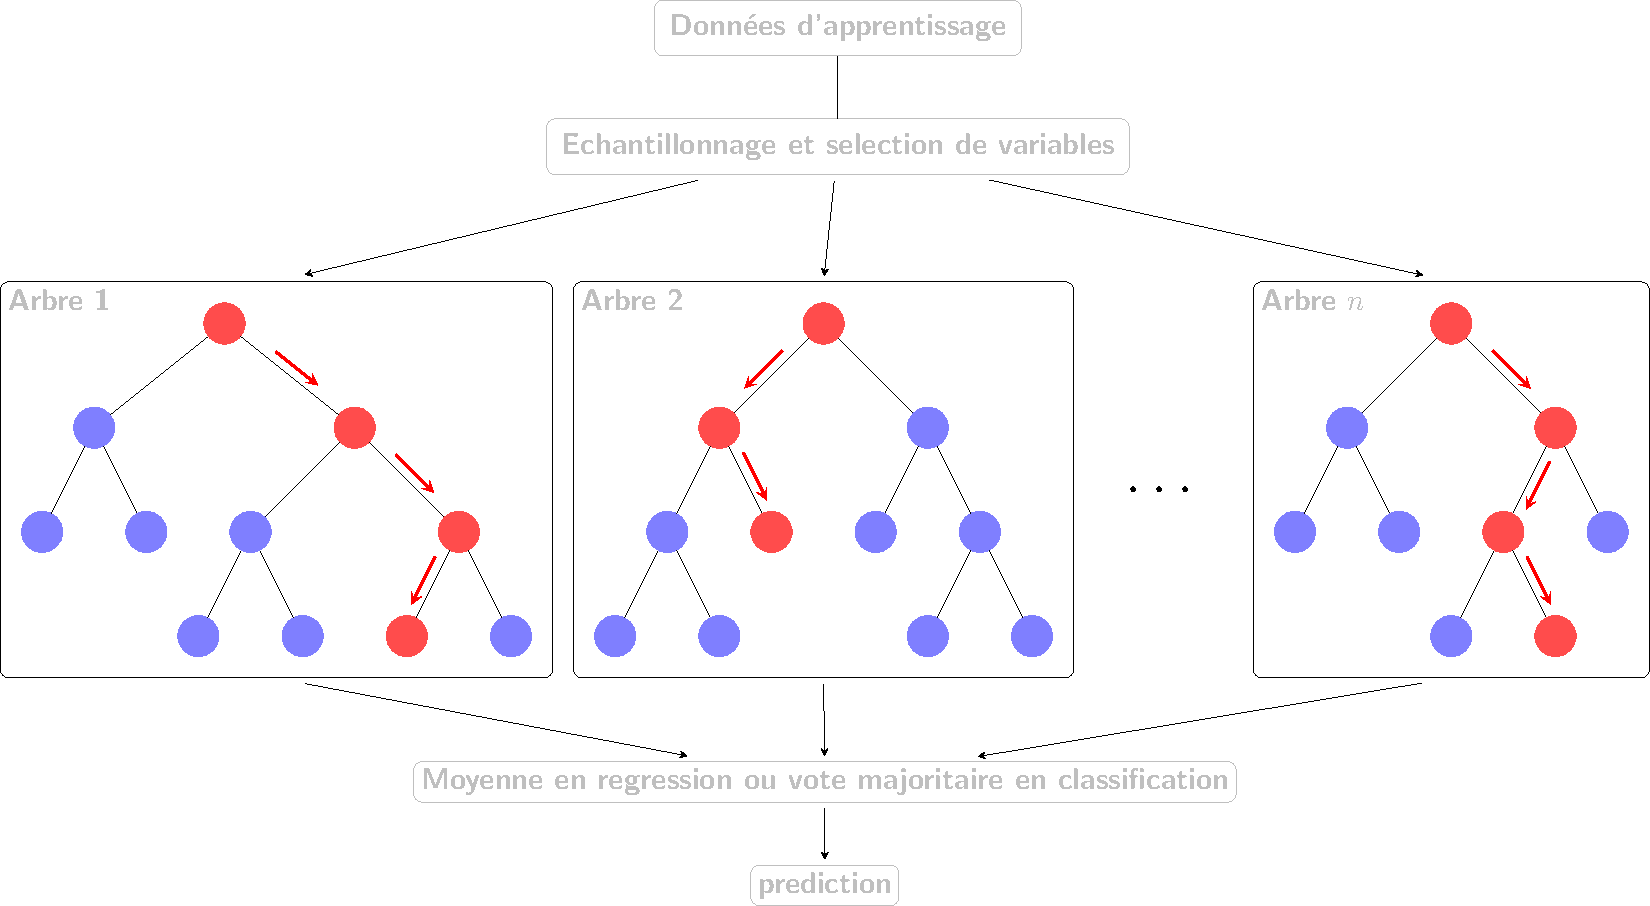
\includegraphics[]{include/random-forest.pdf}}};
  
  
  \node [color=gray!50,rotate=-5]at (.6\textwidth,4){\resizebox{9cm}{5cm}{\def\layersep{2.5cm}

\begin{tikzpicture}[shorten >=1pt,->,draw=black!50, node distance=\layersep]
    \tikzstyle{every pin edge}=[<-,shorten <=1pt]
    \tikzstyle{neuron}=[circle,fill=black!25,minimum size=17pt,inner sep=0pt]
    \tikzstyle{input neuron}=[neuron, fill=green!50];
    \tikzstyle{output neuron}=[neuron, fill=red!50];
    \tikzstyle{hidden neuron}=[neuron, fill=blue!50];
    \tikzstyle{annot} = [text width=4em, text centered]

    % Draw the input layer nodes
    \foreach \name / \y in {1,...,4}
    % This is the same as writing \foreach \name / \y in {1/1,2/2,3/3,4/4}
        \node[input neuron, pin=left:Entrée \#\y] (I-\name) at (0,-\y) {};

    % Draw the hidden layer nodes
    \foreach \name / \y in {1,...,5}
        \path[yshift=0.5cm]
            node[hidden neuron] (H-\name) at (\layersep,-\y cm) {};

    % Draw the output layer node
    \node[output neuron,pin={[pin edge={->}]right:Sortie}, right of=H-3] (O) {};

    % Connect every node in the input layer with every node in the
    % hidden layer.
    \foreach \source in {1,...,4}
        \foreach \dest in {1,...,5}
            \path (I-\source) edge (H-\dest);

    % Connect every node in the hidden layer with the output layer
    \foreach \source in {1,...,5}
        \path (H-\source) edge (O);

    % Annotate the layers
    \node[annot,above of=H-1, node distance=1cm] (hl) {Couche cachée};
    \node[annot,left of=hl] {Couche d'entrée};
    \node[annot,right of=hl] {Couche de sortie};
\end{tikzpicture}}
  };
  
  \node [color=gray!50,rotate= 30]at (1\textwidth,8){\resizebox{7cm}{1.5cm}{{\Large MSE}$\displaystyle= \frac{1}{n}\sum_{i=1}^{n} \left(Y_i -\hat{Y}_{i }\right)^2$}};
  \end{tikzpicture}
};

\end{tikzpicture}


\vspace{-1cm}
%-----------------------------------------------------------------------------------
  %  page de garde
%-----------------------------------------------------------------------------------
  \begin{center}

\begin{large}

\includegraphics[scale=0.3]{Images/le_cnam.png} \\
\textsc{Certificat de spécialisation analyste de données massives}\\ \bigskip
\textbf{ Unité d'enseignement: 
} \end{large}
Entreposage et fouilles de données (STA211)
\end{center}
\bigskip
\shadowoffset{3pt}
\begin{tcolorbox}[blanker,top=1.2cm,bottom=1.2cm,borderline horizontal={4pt}{0pt}{bluePoli},colupper=bluePoli]
\begin{center}
\shadowtext{\resizebox{\textwidth}{1.cm}{{\small Synthèse du cours }}}
\end{center}
\end{tcolorbox}


\bigskip

\begin{minipage}{0.4\textwidth}
\large
\emph{Réalisé par:}\\
\author\\[3mm]
\end{minipage}\\[2cm] 


%\textcolor{bluePoli}{\rule{.82\textwidth}{4pt}\hfill {\fontfamily{pzc}\fontsize{.7cm}{0cm}\selectfont \YEAR }}
\end{titlepage}


\AddToShipoutPicture*{\BackgroundPic}
\small \normalfont

\vspace{11pt}

\centerline{\rule{1.0\textwidth}{0.4pt}}

\begin{center}
\begin{minipage}[t]{.24\textwidth}
\begin{minipage}{.90\textwidth}
\noindent
\scriptsize{\textbf{Professeur:}} \\
\advisor \\
\\
\textbf{Année académique:} \\
\YEAR \\
\\
\end{minipage}
\end{minipage}% This must go next to `\end{minipage}`
\begin{minipage}{.74\textwidth}
\noindent \textbf{\color{bluePoli} Résumé:} {\abstract}
\end{minipage}
\end{center}

\vspace{15pt}

\begin{tcolorbox}[arc=0pt, boxrule=0pt, colback=bluePoli!60, width=\textwidth, colupper=white]
    \textbf{Mots-clés:} \keywords
\end{tcolorbox}

\vspace{12pt}


\section{Définition et contexte d'émergence du data mining}
\subsection{Définition}
Il n'est pas aisé de trouver une définition exacte et claire associé au \textit{data mining}.
Ce que l'on peut retenir c'est le \textit{data mining} désigne un ensemble de méthodes à l'intersection entre plusieurs disciplines (statistiques, intelligence artificielle, informatique,...) permettant d'explorer et d'analyser de grandes bases de données en vue d'extraire des informations utiles.

\par Dans le langage courant, on confond souvent les termes \textit{big data} et \textit{data mining}. Ces deux termes désignent pourtant des choses différentes. 
Le\textit{big data} renvoie à une quantité importante de données. Quand au \textit{data mining}, il désigne l'utilisation des techniques diverses pour extraire de ces énormes quantités de données (big data), de la connaissance utile permettant de tirer un avantage comparative.
\par A partir de quand parle t'on de big data? On parlera de big data quand les techniques traditionnelles de traitement des données ne sont plus opérantes sur les données. Le big data ne se résume pas seulement au seul aspect volumétrie. En effet, le volume est un aspect relatif. En effet avec l'amélioration de capacité de stockage, des données jadis considérées comme volumineuses deviennent moins problèmatiques pour les entreprises.
Le big data est souvent caractérisé par ce qu'on appelle les \textbf{3V}.
Les 3V font référence aux trois aspects suivants: volume, vitesse, variété.
\begin{itemize}
\item \textbf{Le volume} désigne la quantité de données astronomiques générées.
\item \textbf{La vitesse} est la rapidité à laquelle les données sont générées, stockées, transformées et exploitées.
\item \textbf{La variété} fait référence à la diversité des sources de données et leurs types (données structurées, données non-structurées).  Les données prennent le plus souvent des formes très variées et très hétérogènes (son, images, vidéos,textes, etc.)
\end{itemize}
Aux 3V ci-dessus, certains y adjoignent deux autres V pour en faire 5. Ces 2V additionnels sont:
\begin{itemize}
\item La valeur: La valeur désigne la valeur ajoutée 
\item la véracité fait référence à la fiabilité des données 
\end{itemize}
\subsection{Dans quel contexte émergent le data mining?}
Les raisons du succès du data mining s'explique principalement par deux facteurs:
\begin{itemize}
\item L'environnement concurrentiel: La mondialisation a intensifié la concurrence entre les entreprises et saturé les marché. Dans ce environnement de plus en plus concurrentiel le client devient l'acteur principal de l'entreprise. Cela fait naître chez les entreprises le besoin de mieux connaître leurs clients.
\item L'état de l'entreprise: Le développement des systèmes d'informations a entraîné une réduction des coûts de stockages et augmentation des puissances de calcul permettant aux entreprises de stocker et d'exploiter des quantités gigantesques de données.
Avec la concurrence et la disponibilité des données, le besoin de transformer les données d'entreprises en connaissance s'est fait sentir.
Avant toute démarche de data mining il faut être capable de poser de manière clair le problème business auquel on souhaite répondre. Est ce que les données disponibles permettent de répondre à la question qu'on se pose.

Il existe deux types de data mining.
Data mining de vérification et data mining de découverte.
\end{itemize}

\section{Analyse de données}
\subsection{Analyse en composantes principales}

\subsection{Analyse factorielle des correspondances}

\subsection{Analyse des correspondances multiples}


\subsection{Analyse factorielles mixtes}


\begin{knitrout}
\definecolor{shadecolor}{rgb}{0.878, 0.918, 0.933}\color{fgcolor}\begin{kframe}
\begin{alltt}
\hlkwd{library}\hlstd{(dplyr)}
\hlkwd{library}\hlstd{(tidyverse)}
\hlkwd{library}\hlstd{(FactoMineR)}
\hlkwd{library}\hlstd{(missMDA)}
\hlkwd{library}\hlstd{(caret)}
\end{alltt}
\end{kframe}
\end{knitrout}

\begin{knitrout}
\definecolor{shadecolor}{rgb}{0.878, 0.918, 0.933}\color{fgcolor}
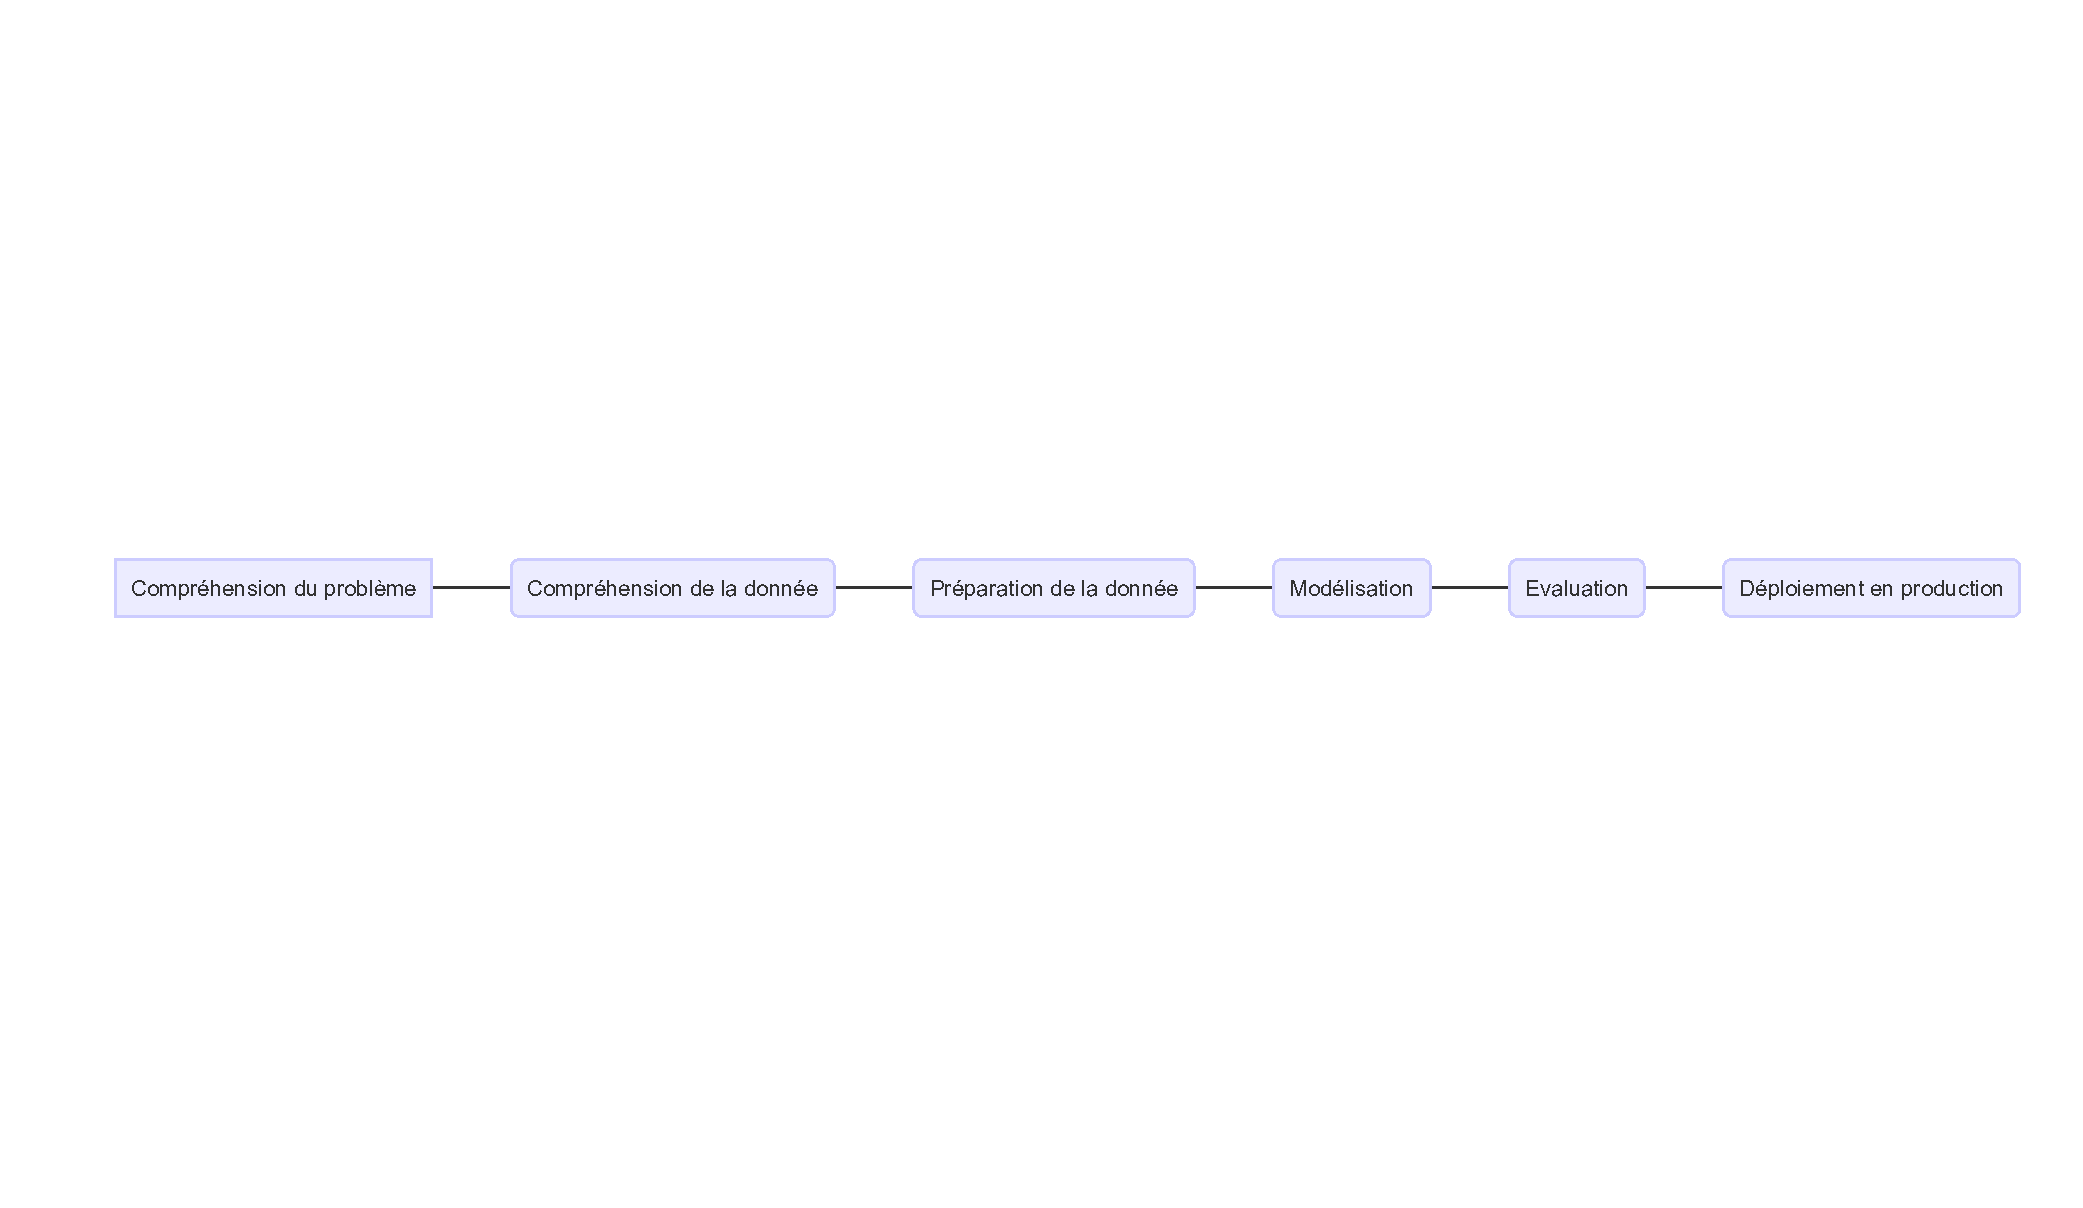
\includegraphics[width=\maxwidth]{figure/unnamed-chunk-3-1} 
\end{knitrout}




\section{SVM}
Les supports vecteurs machines
\section{Business intelligence avec BO}

\bibliography{bibliography.bib}

\end{document}
